\section{Collision Avoidance} \label{sec:collision_avoidance}

% \subsection{Disturbance Repulsion}
The principal goal of the controller introduced in the previous section is its ability to ensure collision avoidance in the presence of external disturbances.
However, the control force $\vect \tau^c$ proposed in \eqref{eq:control_command} does not explicitly consider external forces. Yet, it is designed to correct the agent's velocity $\dot{\vecs \xi}$ if it deviates from the desired velocity $\ddot{\vecs \xi}$.\footnote{Note that for a discrete-time (digital) controller, this results in a delay.}

Since interaction with the environment results in a force on the system, often over a short period $\Delta t \ll 1$.  Hence, we can define the velocity after impact $\vect v^I$ as:
\begin{align}
	 % \begin{split}
	\vect v^I
	  \approx \int_{t^I}^{t^I + \Delta t} \ddot{\vecs \xi} dt  
	  \approx \int_{t^I}^{t^I + \Delta t} \matd{M}^{-1}(\vecs \xi)  \vecs \tau_e \, dt  
	 % \end{split}
	  \label{eq:impact_velocity}
\end{align}
using the controller from \eqref{eq:robot_dynamics}, and under absence of the control force $\vecs \tau_c$ during this short timeframe. Additionally, $\{\vect \xi \}_{t^I}$ is the velocity before the impact.
 
% Since the magnitude of the normal is limited to $1$, the control weight is limited as: 
% \begin{equation}
% w(\vecs \xi) \geq \frac{\Gamma^{\mathrm{crit}} - \Gamma(\vecs \xi)}{\Gamma^{\mathrm{crit}} - 1}
% \end{equation}
% under the assumption that $\Gamma^{\mathrm{crit}} \geq 1$.

% Using the controller design from \eqref{eq:control_command} the velocity can be computed as:
% \begin{equation}
% \begin{split}
% 	\{ \vecs{\dot \xi} \}_{t} 
% 	& = \int \vecs{\ddot \xi} \, dt = \int \matd{M}^{-1} \matd{D}  \bigl( \vecs{\dot \xi} - \vecs f(\vecs \xi) \bigr) \, dt \\
% 	& = \int \matd{M}^{-1} \matd{D} \bigl( \vecs{\dot \xi} - \vecs f(\vecs \xi) \bigr) \, dt \\
% 	& = \matd{M}^{-1} \int \left( (1 - w) \matd{D}^f + w \matd{D}^{o} \right)  \bigl( \dot{\vecs \xi} - \vecs f(\vecs \xi) \bigr) dt\\
% 	& = \matd{M}^{-1} \int  \matd{D}\bigl( \vecs \xi - t \vecs f(\vecs \xi) \bigr) + C_t \\
% 	% &  \underset{}\{ {\vecs \xi} \}_0 = \vecs f(\vecs \xi) + \vecs v^I{=} \matd{M}^{-1} \matd{D}  \left( \xi - t \vecs f(\vecs \xi) \right) + C_t \\
% 	&  = \matd{M}^{-1} \matd{D}  \bigl( \vecs \xi - \{\vecs \xi\}_0  - t \vecs f(\vecs \xi) \bigr) + \vecs f(\vecs \xi) + \vecs v^I \\
%     % & \approx \int \matd{M}^{-1} \matd{D} \vect f(\vecs \xi) \, dt
% \end{split}
% \label{eq:velocity_evolution}
% \end{equation}
% using $\{ {\vecs \xi} \}_0 = \vecs f(\vecs \xi) + \vecs v^I$ to find the integration constant $C_t$.

Furthermore, let us consider a desired velocity $\vect f(\vecs \xi)$, which is a constant, collision-free vector field parallel to the surface of a flat obstacle surface (see Fig.~\ref{fig:disturbance_with_parallel_velocity}):
\begin{equation}
	\dotprod{\vect f(\vecs \xi)}{\vecs n(\vecs \xi)} = 0
	 \qquad
\vect f(\vecs \xi) = \text{const.}
\, , \;
\vect n(\vecs \xi) = \text{const.}
\label{eq:parallel_velocity}
\end{equation}
where $\vecs n(\vecs \xi)$ is the surface's normal vector, and the agent moves in a straight line, hence we can neglect the Coriolis effect. For disturbances in such environments, we show that our approach can ensure the impenetrability of the obstacle up to an upper bound on the magnitude of the disturbance:

\begin{lemma} \label{lemma:damping_collision_avoidance}
	Consider a point-mass agent with mass $m \in \mathbb{R}_{>0}$, whose motion evolves according to the rigid body dynamics given in \eqref{eq:robot_dynamics} controlled by \eqref{eq:control_command}, with constant damping matrix $\matd{D}$ from \eqref{eq:damping_summation}. The agent tracks a constant reference velocity ${\mathrm{f}}$, whose vector field moves parallel to a flat obstacle as given in \eqref{eq:parallel_velocity}. Any motion path initiated in free space will remain collision-free for all times, i.e., $\Gamma( \{\vecs \xi_t\}) \geq 1$ with $t \geq 0$ if the impact velocity $v^I$ as given in \eqref{eq:impact_velocity} at time $t=0$ is limited by $\| \vect v^I\| < s^{\mathrm{f}} \| \vecs \xi - \vecs \xi^b \| / m$, with respect to the closest surface point $\vecs \xi^b \in \mathbb{R}^N$.
\end{lemma}

% \begin{lemma}
% 	A dynamical system evolves with the rigid body dynamics given in \eqref{eq:robot_dynamics} controlled by \eqref{eq:control_command}, with damping matrix $\matd{D}$ from \eqref{eq:damping_summation}, and a negligible Coriolis effect.
%     A point-like agent starting at position $\vect p = \{{\vecs \xi}\}_0$ close to the surface, i.e., $\Gamma( \vect p) \approx 1$ is guided by a velocity field $\vect f(\vecs \xi)$ parallel to the surface with a starting velocity $\vect v^0= \vect f(\{{\vecs \xi}\}_0)$.
%     A large disturbance towards the obstacle results in a velocity of $\{\dot{\vecs \xi}\}_0 = \vect v^I +  \vect v^0$ after the impact, with $\| \vect v^I \| \gg \| \vect v^0 \|$.
% 	A motion starting in free space remains collision-free for all times, i.e., $\Gamma( \{\vecs \xi_t\}) \geq 1$ with $t \geq 0$ if the impact velocity is limited by $\| \vect v^I\| < s^{\mathrm{o}} \| \vecs \xi - \vecs \xi^b \| / m^{\mathrm{min}}$, with respect to the closes surface point $\vecs \xi^b \in \mathbb{R}^N$ and mass $m \in \mathbb{R}_{>0}$.
% \end{lemma}

\begin{proof}
According to the Bony-Bezis theorem \parencite{bony1969principe}, the trajectories are collision-free if there is zero velocity towards the obstacle on the surface, i.e.,
\begin{equation}
	\left| \vect n(\vecs \xi)^T \, \{ \vecs{\dot \xi} \}_{t} \right| = 0 
	\quad \forall \, \Gamma(\vecs \xi) = 1
	\label{eq:bezis_theorem}
\end{equation}

We want to find the time when the agent stops moving towards the obstacle, enabling us to evaluate the distance traveled as a function of the velocity after disturbance $\vect v^I$. 
Let us assume without loss of generality that the disturbance occurs at time $t=0$. Hence, the velocity at time $T$ can be computed as:
\begin{equation}
\begin{split}
	\{ \vecs{\dot \xi} \}_{T} 
	& = \int_0^T \vecs{\ddot \xi} \, dt = \int_0^T \matd{M}^{-1} \matd{D} \left( \vecs{\dot \xi} - \vect f(\vecs \xi ) \right) \, dt \\
	& = \matd{M}^{-1} \int \left( (1 - w) \matd{D}^f + w \matd{D}^{o} \right) \left( \vecs{\dot \xi} - \vect f (\vecs \xi ) \right) dt \\
	\end{split}
\label{eq:velocity_evolution}
\end{equation}

Furthermore, since the vector field, $\vect f(\vecs \xi)$ is constant and the obstacle's surface does not have any curvature, it follows from \eqref{eq:damping_summation} that the damping matrices  $\matd{D}^o$ and $\matd{D}^f$ are constant.
Moreover, by design of the damping matrices, from \eqref{eq:first_obstacle_basis} it follow that $\matd{D}^o(\vecs \xi) \vect n(\vecs \xi) = s^o \vect n(\vecs \xi)$, and from  \eqref{eq:velocity_unit_vector} that $\matd{D}^f(\vecs \xi) \vect n(\vecs \xi) = s^f \vect n(\vecs \xi)$. 

From \eqref{eq:bezis_theorem} follows that it is sufficient to observe the normal component of the vectors only. Thus, in the rest of this paragraph, the components along the normal are denoted by scalar values, e.g. $\dot \xi = \dotprod{\dot{\vecs \xi}}{\vecs n(\vecs \xi)} \vecs n(\vecs \xi)$.
Hence, we get:
\begin{align}
	0 & = \left| \vect n(\vecs \xi)^T \, \{ \vecs{\dot \xi} \}_{t} \right| 
	  = \frac 1 m \int_0^T ( (1-w) \vect n^T \matd{D}^f \vect n + w s^{o} ) \, {\dot \xi} \, dt \nonumber \\
	   & < \frac 1 m \int_0^T  s^{f}  \, {\dot \xi} \, dt 
	   = \frac{s^f}{m} (\xi - \{ \xi \}_0 ) + v^I \, dt 
\end{align}
where $m = \max{\left(\text{eig}(\matd{M})\right)}$, with the maximum displacement as:
\begin{equation}
	\| \{\xi \}_0 - {\xi} \| \leq \| v^I \| {m} / {s^{\mathrm{f}}} 
\end{equation}
% To see when the differences reaches zero, we can compute
% \begin{equation}
%  \|	\{ \vecs{\dot \xi} \}_T - \vect f(\vecs \xi) \| = 0
%  \quad \Rightarrow \quad
%     \| \vecs{\xi}_1 -  \vect p_1 \| = \| \vecs v^I_1 \| {m} / {s^{\mathrm{o}}} 
%  \end{equation}
\end{proof}

Lemma~\ref{lemma:damping_collision_avoidance} assumes constant velocity field $\vect f(\vecs \xi)$ and flat obstacle surface. This is an appropriate assumption for large velocities after disturbances towards the obstacle, i.e., $\| \vect v^I \| \gg \| \vect f(\vecs \xi) \|$ and starting close to the surface. Since the distance traveled has to be flat to avoid collision, the vectorfield is likely to show small changes, and the surface has little deviation. 

\begin{figure}[htb]
\centering
 % \begin{subfigure}{0.99\columnwidth}
  \centerline{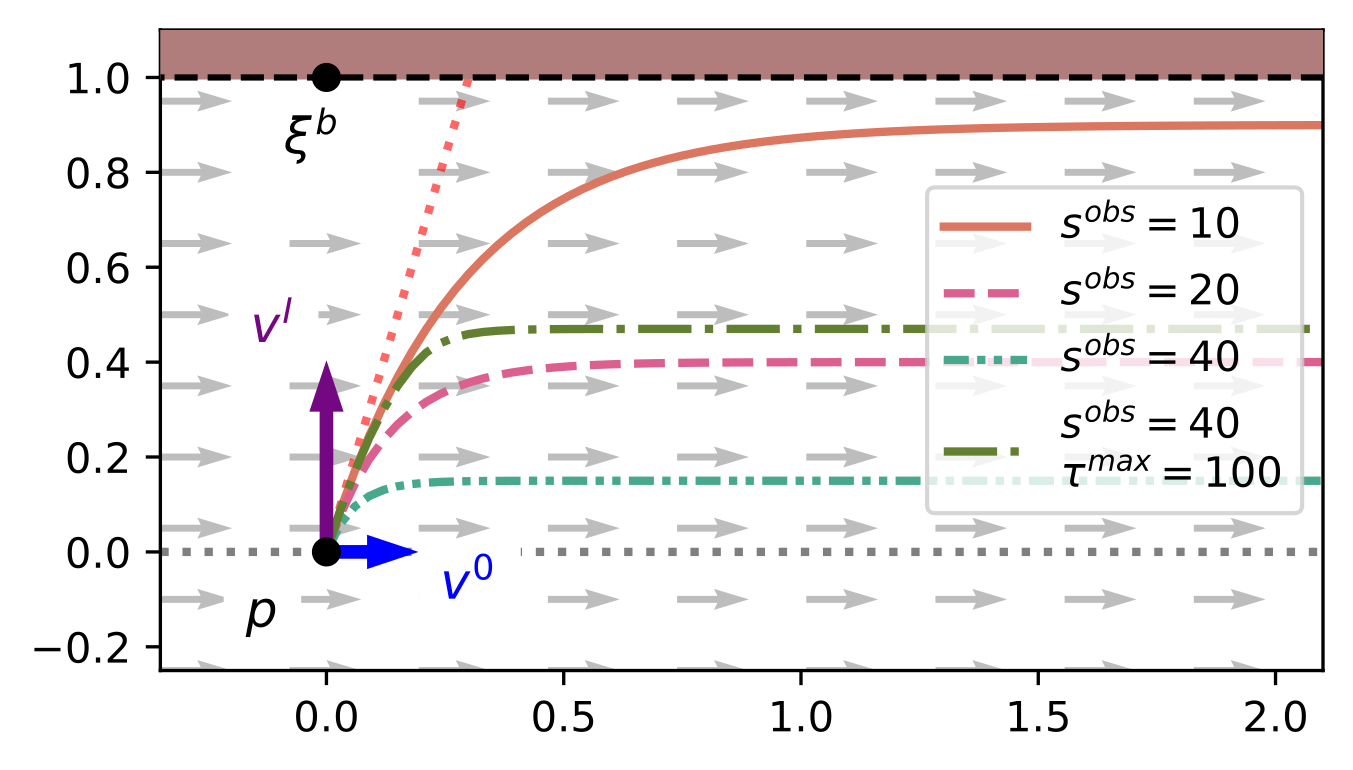
\includegraphics[width=0.99\columnwidth]{figures/parallel_avoidance_obstacle}}
  \caption{A disturbance occurs of a point-agent at position $\vect p^0$ with velocity after the impact of $\{ \dot{\vecs \xi} \}_0 = \vect v^0 + \vect v^I$. A high damping in the direction of the obstacle in the presence of a constant velocity field (gray) ensures collision avoidance. Whereas different damping values $s^{\mathrm{o}}$ and optionally a maximum repulsion force $\vecs \tau^{\mathrm{max}}$ lead to different trajectories.}
  \label{fig:disturbance_with_parallel_velocity}
% \end{subfigure}
\end{figure}
    
Nevertheless, there is no guarantee against drifting into obstacles in the presence of highly curved surfaces and velocity fields. \iflong This is further discussed during the experiments in Section~\ref{sec:position_noise}, where the increased damping towards the obstacle significantly reduces collision in such scenarios. \fi However, designing a repulsive field as proposed in \parencite{huber2023avoidance} can ensure collision avoidance in such scenarios.

\iflong
% \subsection{Disturbance Repulsion with Force Limit}
All robotic systems have a maximum force that they can exert on the environment based on the motors, geometry, and state, $\tau_c^{\mathrm{max}} \in \mathbb{R}_{>0}$. Such a limiting force decreases the impact velocity a controller can handle while ensuring collision avoidance, as shown in Fig.~\ref{fig:disturbance_with_parallel_velocity}. Nevertheless, a maximum control force can be interpreted as adapting damping; hence, the passivity from Theorem~\ref{theorem:passivity} holds.
\fi

